\chapter{Evalutation}
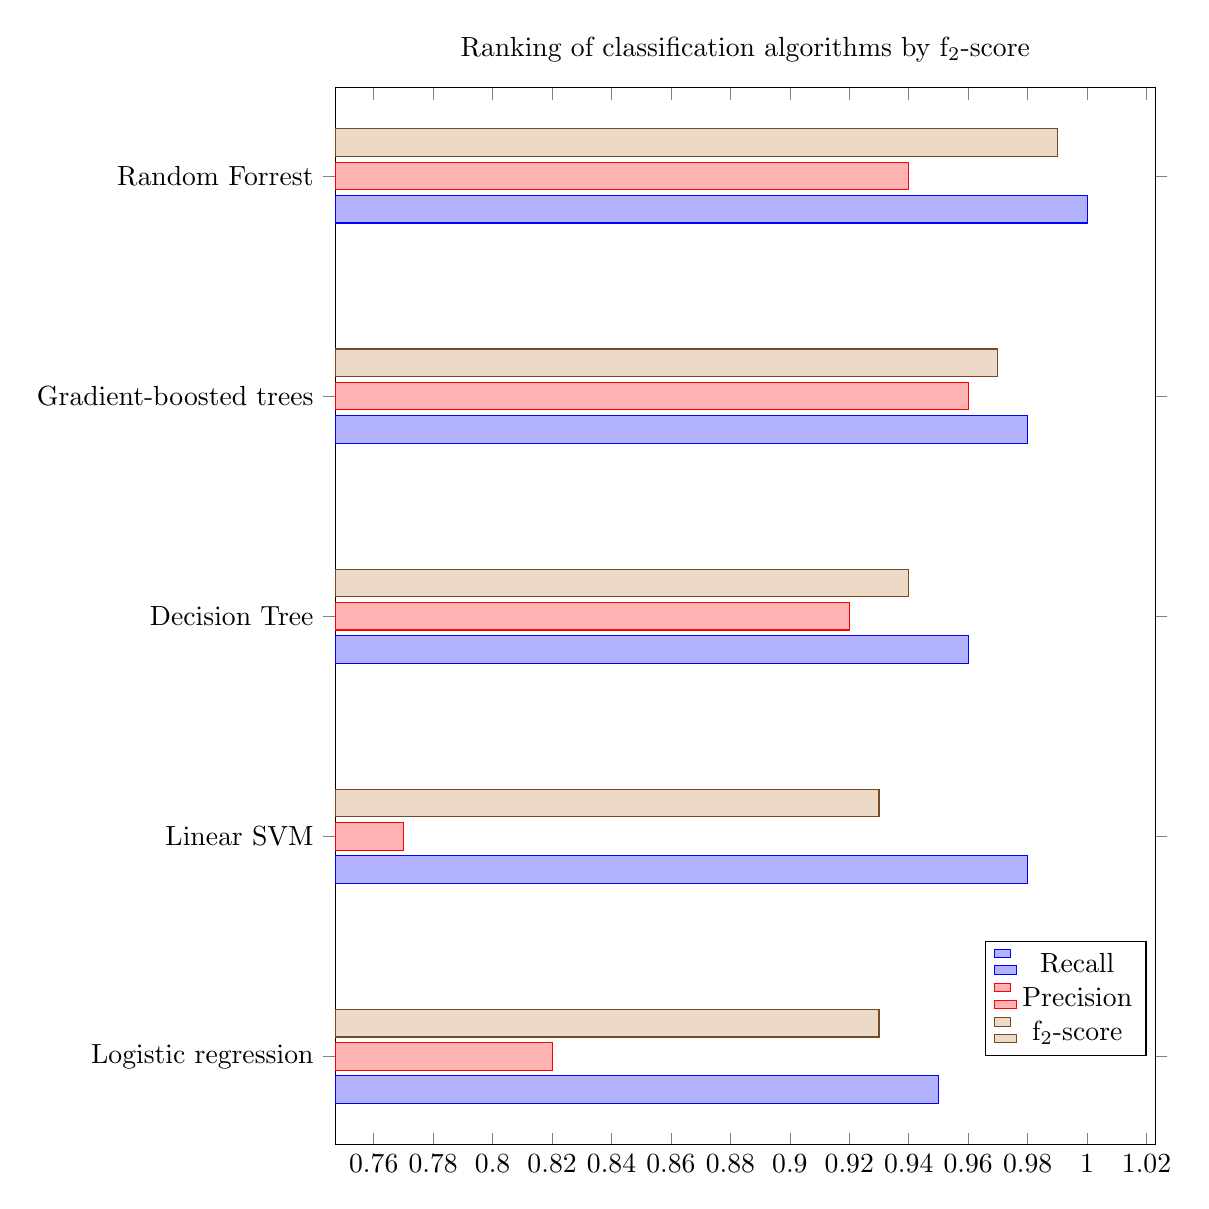
\begin{tikzpicture}
\begin{axis}[
title=Ranking of classification algorithms by f\textsubscript{2}-score,
xbar,
enlarge y limits=0.5,
%xlabel={f\textsubscript{2}-score},
width=12cm, height=15cm, enlarge y limits=0.1,
symbolic y coords={
%Naiv bayes
Logistic regression,
Linear SVM,
Decision Tree,
Gradient-boosted trees,
Random Forrest
},
ytick=data,
legend style={at={(axis cs:1.02,Logistic regression)},anchor=south east}
]

\addplot coordinates {
(1.00,Random Forrest)
(0.98,Linear SVM)
(0.95,Logistic regression)
(0.96,Decision Tree)
(0.98,Gradient-boosted trees)
%(0.97,Naiv Bayes)
};
\addplot coordinates {
(0.94,Random Forrest)
(0.77,Linear SVM)
(0.82,Logistic regression)
(0.92,Decision Tree)
(0.96,Gradient-boosted trees)
%(0.97,Naiv Bayes)
};
\addplot coordinates {
(0.99,Random Forrest)
(0.93,Linear SVM)
(0.93,Logistic regression)
(0.94,Decision Tree)
(0.97,Gradient-boosted trees)
%(0.97,Naiv Bayes)
};

\legend{Recall, Precision, f\textsubscript{2}-score}
\end{axis}
\end{tikzpicture}